\documentclass{article}\usepackage[]{graphicx}\usepackage[]{color}
%% maxwidth is the original width if it is less than linewidth
%% otherwise use linewidth (to make sure the graphics do not exceed the margin)
\makeatletter
\def\maxwidth{ %
  \ifdim\Gin@nat@width>\linewidth
    \linewidth
  \else
    \Gin@nat@width
  \fi
}
\makeatother

\definecolor{fgcolor}{rgb}{0.345, 0.345, 0.345}
\newcommand{\hlnum}[1]{\textcolor[rgb]{0.686,0.059,0.569}{#1}}%
\newcommand{\hlstr}[1]{\textcolor[rgb]{0.192,0.494,0.8}{#1}}%
\newcommand{\hlcom}[1]{\textcolor[rgb]{0.678,0.584,0.686}{\textit{#1}}}%
\newcommand{\hlopt}[1]{\textcolor[rgb]{0,0,0}{#1}}%
\newcommand{\hlstd}[1]{\textcolor[rgb]{0.345,0.345,0.345}{#1}}%
\newcommand{\hlkwa}[1]{\textcolor[rgb]{0.161,0.373,0.58}{\textbf{#1}}}%
\newcommand{\hlkwb}[1]{\textcolor[rgb]{0.69,0.353,0.396}{#1}}%
\newcommand{\hlkwc}[1]{\textcolor[rgb]{0.333,0.667,0.333}{#1}}%
\newcommand{\hlkwd}[1]{\textcolor[rgb]{0.737,0.353,0.396}{\textbf{#1}}}%
\let\hlipl\hlkwb

\usepackage{framed}
\makeatletter
\newenvironment{kframe}{%
 \def\at@end@of@kframe{}%
 \ifinner\ifhmode%
  \def\at@end@of@kframe{\end{minipage}}%
  \begin{minipage}{\columnwidth}%
 \fi\fi%
 \def\FrameCommand##1{\hskip\@totalleftmargin \hskip-\fboxsep
 \colorbox{shadecolor}{##1}\hskip-\fboxsep
     % There is no \\@totalrightmargin, so:
     \hskip-\linewidth \hskip-\@totalleftmargin \hskip\columnwidth}%
 \MakeFramed {\advance\hsize-\width
   \@totalleftmargin\z@ \linewidth\hsize
   \@setminipage}}%
 {\par\unskip\endMakeFramed%
 \at@end@of@kframe}
\makeatother

\definecolor{shadecolor}{rgb}{.97, .97, .97}
\definecolor{messagecolor}{rgb}{0, 0, 0}
\definecolor{warningcolor}{rgb}{1, 0, 1}
\definecolor{errorcolor}{rgb}{1, 0, 0}
\newenvironment{knitrout}{}{} % an empty environment to be redefined in TeX

\usepackage{alltt}
\title{Stat159 Project 3: Add a title}
\author{Liang Hao, Bret Hart, Andrew Shibata, Gary Nguyen}
\date{\today}
\IfFileExists{upquote.sty}{\usepackage{upquote}}{}
\begin{document}

\maketitle
\section{Data}



\subsection{Description}

The data we used for this project come from the *College Scorecard* , which is developed by the U.S. Department of Education (under Obama's Administration) to provide "key indicators about the cost and value of institutions across the country to help students choose a school that is well-suited to meet their needs, priced affordably, and is consistent with their educational and career goals". The link to the data can be found [here](https://collegescorecard.ed.gov/data/). For now, the (website)[https://collegescorecard.ed.gov/] provides basic information about facts about educational institutions upon search. 

\subsection{Cleaning}
For our purpose, we collect the raw data for the past five years, and clean up in the following way:

1: For dataset of each of the five years, we get the columns and rows with less than 10% *PrivacySuppressed* or *NaN*, in order to obtain a data set with sufficient information. And we take the intersection of the columns and rows as our first step. Such process leaves us with around around 600 columns and around 6700 colleges.

2: Then we run through the data dictionary to extract useful columns that may help in building model and the shiny App for this project. The process decreases the number of columns to under 300.

3: We parse the five dataset with the selected columns and rows.

4: Believing that closer years have more value as information, we combine the five dataset with the following weight:

\begin{table}[ht]
\centering
\begin{tabular}{rrrrrr}
  \hline
 & Year 2014-2015 & Year 2013-2014 & Year 2012-2013 & Year 2011-2012 & Year 2010-2011 \\ 
  \hline
Weight & 0.40 & 0.30 & 0.10 & 0.05 & 0.05 \\ 
   \hline
\end{tabular}
\end{table}


5: Lastly, we merge the combined dataset with the *Post-Graduation Salary* dataset to form the data frame to be used in this project. 

\subsection{Exploratory Data Analysis}

\subsubsection{Geographical Distribution}
We may first have a look at the geographical distribution of colleges in the dataset. For the purpose of graphing, the plot only shows colleges in mainland United States.

\begin{knitrout}
\definecolor{shadecolor}{rgb}{0.969, 0.969, 0.969}\color{fgcolor}

{\centering 
\includegraphics[width=300px]{../images/ggplot-schoolDistribution} 

}



\end{knitrout}

We may see that blablablablabla


Then, we may look at the 
\begin{knitrout}
\definecolor{shadecolor}{rgb}{0.969, 0.969, 0.969}\color{fgcolor}

{\centering 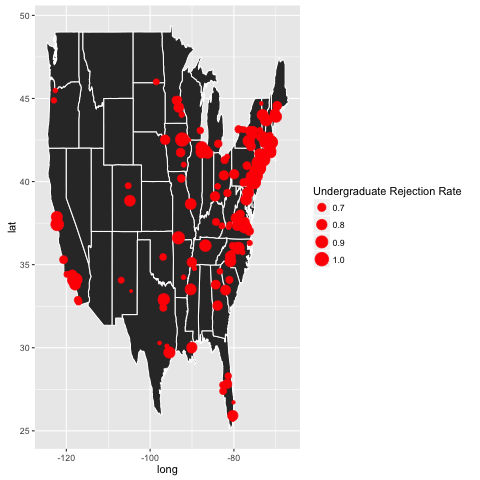
\includegraphics[width=300px]{../images/ggplot-admissionRateDistribution} 

}



\end{knitrout}

\subsubsection{Ethnicity}

We can also look at the historical statistics for educational conditions for minority groups. For such causes have long been drawing attention from the society and the public still complain about it.
\begin{table}[ht]
\centering
\begin{tabular}{rlrr}
  \hline
 & HBCU & Frequency & RelativeFrequency \\ 
  \hline
1 & No & 6613 & 0.98 \\ 
  2 & Yes & 102 & 0.02 \\ 
   \hline
\end{tabular}
\caption{Flag for Historically Black College and University} 
\end{table}
\begin{table}[ht]
\centering
\begin{tabular}{rlrr}
  \hline
 & PBI & Frequency & RelativeFrequency \\ 
  \hline
1 & No & 6622 & 0.99 \\ 
  2 & Yes &  93 & 0.01 \\ 
   \hline
\end{tabular}
\caption{Flag for predominantly Black Institution} 
\end{table}
\begin{table}[ht]
\centering
\begin{tabular}{rlrr}
  \hline
 & ANNHI & Frequency & RelativeFrequency \\ 
  \hline
1 & No & 6680 & 0.99 \\ 
  2 & Yes &  35 & 0.01 \\ 
   \hline
\end{tabular}
\caption{Flag for Alaska Native, Native Hawaiian Serving Institution} 
\end{table}
\begin{table}[ht]
\centering
\begin{tabular}{rlrr}
  \hline
 & HSI & Frequency & RelativeFrequency \\ 
  \hline
1 & No & 6368 & 0.95 \\ 
  2 & Yes & 347 & 0.05 \\ 
   \hline
\end{tabular}
\caption{Flag for Hispanic-Serving Institution} 
\end{table}
\begin{table}[ht]
\centering
\begin{tabular}{rlrr}
  \hline
 & TRIBAL & Frequency & RelativeFrequency \\ 
  \hline
1 & No & 6684 & 1.00 \\ 
  2 & Yes &  31 & 0.00 \\ 
   \hline
\end{tabular}
\caption{Flag for Tribal College and University} 
\end{table}
\begin{table}[ht]
\centering
\begin{tabular}{rlrr}
  \hline
 & AANAPII & Frequency & RelativeFrequency \\ 
  \hline
1 & No & 6586 & 0.98 \\ 
  2 & Yes & 129 & 0.02 \\ 
   \hline
\end{tabular}
\caption{Flag for Asian American, Native American, Pacific Islander-serving Institution} 
\end{table}


From the tables above, we can see that the minority groups are under-represented in most of the educational institutions in the U.S.. We may also look at the tthniticy of total share of enrollment of undergraduate degree-seeking students in the dataset.

\begin{knitrout}
\definecolor{shadecolor}{rgb}{0.969, 0.969, 0.969}\color{fgcolor}

{\centering 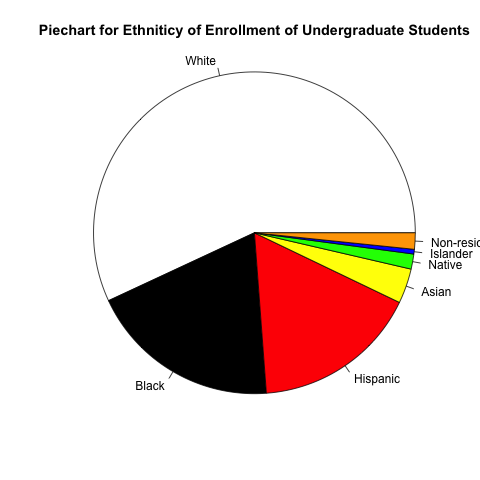
\includegraphics[width=250px]{../images/piechart-enrollmentEthnicity} 

}



\end{knitrout}

From the pie chart above, we may see that ..............................

\subsubsection{Net Price}
Net price is the ....................

\begin{table}[ht]
\centering
\begin{tabular}{rrrrrrrrrr}
  \hline
 & Min. & Max. & Range & Median & 25th & 75th & IQR & Mean & SD \\ 
  \hline
Public & 126.32 & 27055.80 & 26929.48 & 8604.50 & 6217.02 & 12397.31 & 6180.28 & 9444.23 & 4466.77 \\ 
  Private & 639.00 & 74245.42 & 73606.42 & 18337.28 & 13233.46 & 22543.12 & 9309.66 & 18143.31 & 7037.34 \\ 
   \hline
\end{tabular}
\caption{Summary Statistics for Net Price of Public and Private Institutions} 
\end{table}


From the table above, we can see that ............................


\subsubsection{Standardized Test Scores}

The Standardized Test Scores could be important indications for the quality of school and how likely a student may get admission. So we may look at the general distribution of SAT and ACT scores.



{\centering 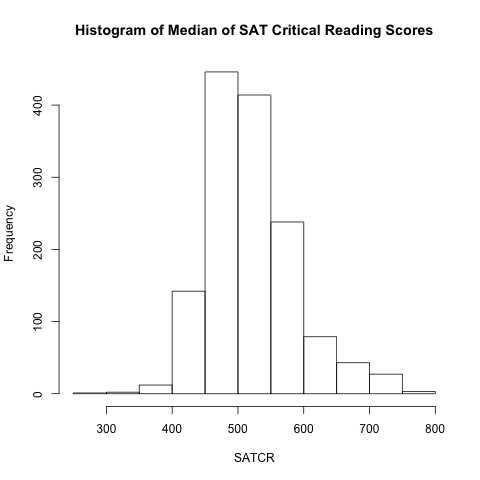
\includegraphics[width=150px]{../images/histogram-SATCRMedian} 

}


\begin{table}[ht]
\centering
\begin{tabular}{rrrrrrrrrr}
  \hline
 & Min. & Max. & Range & Median & 25th & 75th & IQR & Mean & SD \\ 
  \hline
1 & 298.00 & 757.25 & 459.25 & 511.50 & 475.50 & 556.25 & 80.75 & 520.90 & 66.81 \\ 
   \hline
\end{tabular}
\caption{Summary Statistics for SAT Critical Writing} 
\end{table}


From the histogram and the table above, we can see that the median of SAT Critical Reading scores basically follows a normal distribution, with most of the scores clustering between 450 and 550. We may consider colleges with such score higher than 556 to be outstanding as a college institution.



{\centering 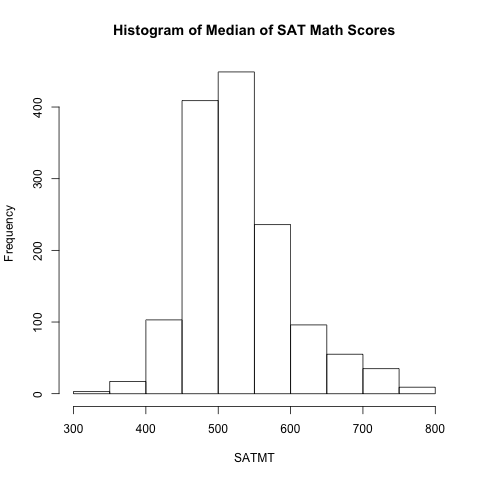
\includegraphics[width=150px]{../images/histogram-SATMTMedian} 

}


\begin{table}[ht]
\centering
\begin{tabular}{rrrrrrrrrr}
  \hline
 & Min. & Max. & Range & Median & 25th & 75th & IQR & Mean & SD \\ 
  \hline
1 & 305.00 & 783.75 & 478.75 & 516.00 & 482.31 & 563.17 & 80.86 & 528.66 & 70.38 \\ 
   \hline
\end{tabular}
\caption{Summary Statistics for SAT Math} 
\end{table}


From the histogram and the table above, we can see that the median of SAT Mathematics scores basically follows a normal distribution, with most of the scores clustering between 450 and 550. We may consider colleges with such score higher than 563 to be outstanding as a college institution.

Because not all colleges recorded or submitted their SAT Writing scores to the original dataset, we may remove in the consideration. Also, we may conduct similar analysis on reported ACT scores:



{\centering 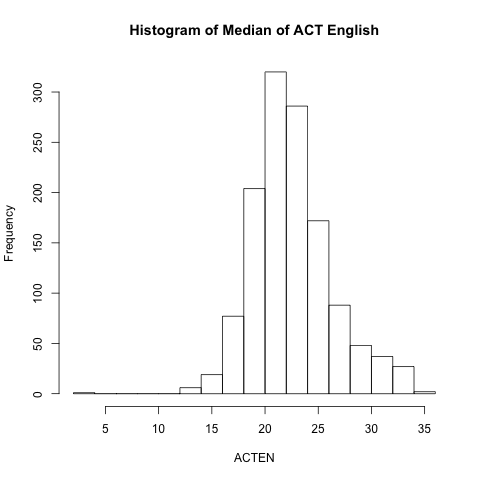
\includegraphics[width=150px]{../images/histogram-ACTENMedian} 

}


\begin{table}[ht]
\centering
\begin{tabular}{rrrrrrrrrr}
  \hline
 & Min. & Max. & Range & Median & 25th & 75th & IQR & Mean & SD \\ 
  \hline
1 & 2.00 & 34.40 & 32.40 & 22.17 & 20.16 & 24.60 & 4.44 & 22.69 & 3.78 \\ 
   \hline
\end{tabular}
\caption{Summary Statistics for ACT English} 
\end{table}


From the histogram and the table above, we can see that the median of ACT English scores basically follows a normal distribution, with most of the scores clustering between 20 and 24. We may consider colleges with such score higher than 24.6 to be outstanding as a college institution.



{\centering 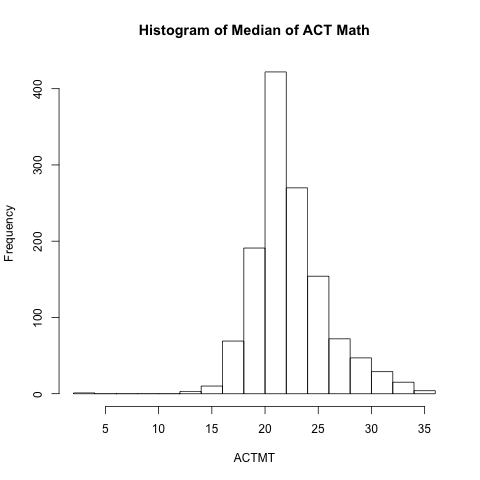
\includegraphics[width=150px]{../images/histogram-ACTMTMedian} 

}


\begin{table}[ht]
\centering
\begin{tabular}{rrrrrrrrrr}
  \hline
 & Min. & Max. & Range & Median & 25th & 75th & IQR & Mean & SD \\ 
  \hline
1 & 2.00 & 35.40 & 33.40 & 21.95 & 20.40 & 24.00 & 3.60 & 22.47 & 3.41 \\ 
   \hline
\end{tabular}
\caption{Summary Statistics for ACT Math} 
\end{table}


From the histogram and the table above, we can see that the median of ACT Math scores basically follows a normal distribution, with most of the scores clustering between 20 and 24. We may consider colleges with such score higher than 24 to be outstanding as a college institution.


\end{document}
